\documentclass[a4paper]{article}

\usepackage{url}
\usepackage{graphicx}	% For figure environment
\usepackage{epstopdf}
\usepackage[center]{subfigure}
\usepackage{amssymb}	% For mathematical figures like \mathbb{R}
\usepackage{amsmath}
\usepackage{framed}
\usepackage{tikz}
\usetikzlibrary{mindmap,trees}
\usepackage{pdflscape}
\usepackage[a4paper]{geometry}


\title{Advanced Systems Lab - Milestone I} 
\author{Lukas Elmer, Matthias Ganz} 
\date{\today} 


\begin{document}

\maketitle


\begin{abstract}

This document, describes the message queuing system which was build. Architecture and design choices are shown and explained. Further test scenarios and test loads are defined. Resulting test output is described and analysed.

\end{abstract}

%% %%%%%%%%%%%%%%%%%%%%%%%%%%%%%%%%%%%%%%%%%%%%%%
\section{Messaging System}
In this section the system under test (or middle ware component) is described.


%% ----------------------------------------------
\subsection{Overview}

\begin{figure}
  \begin{center}
    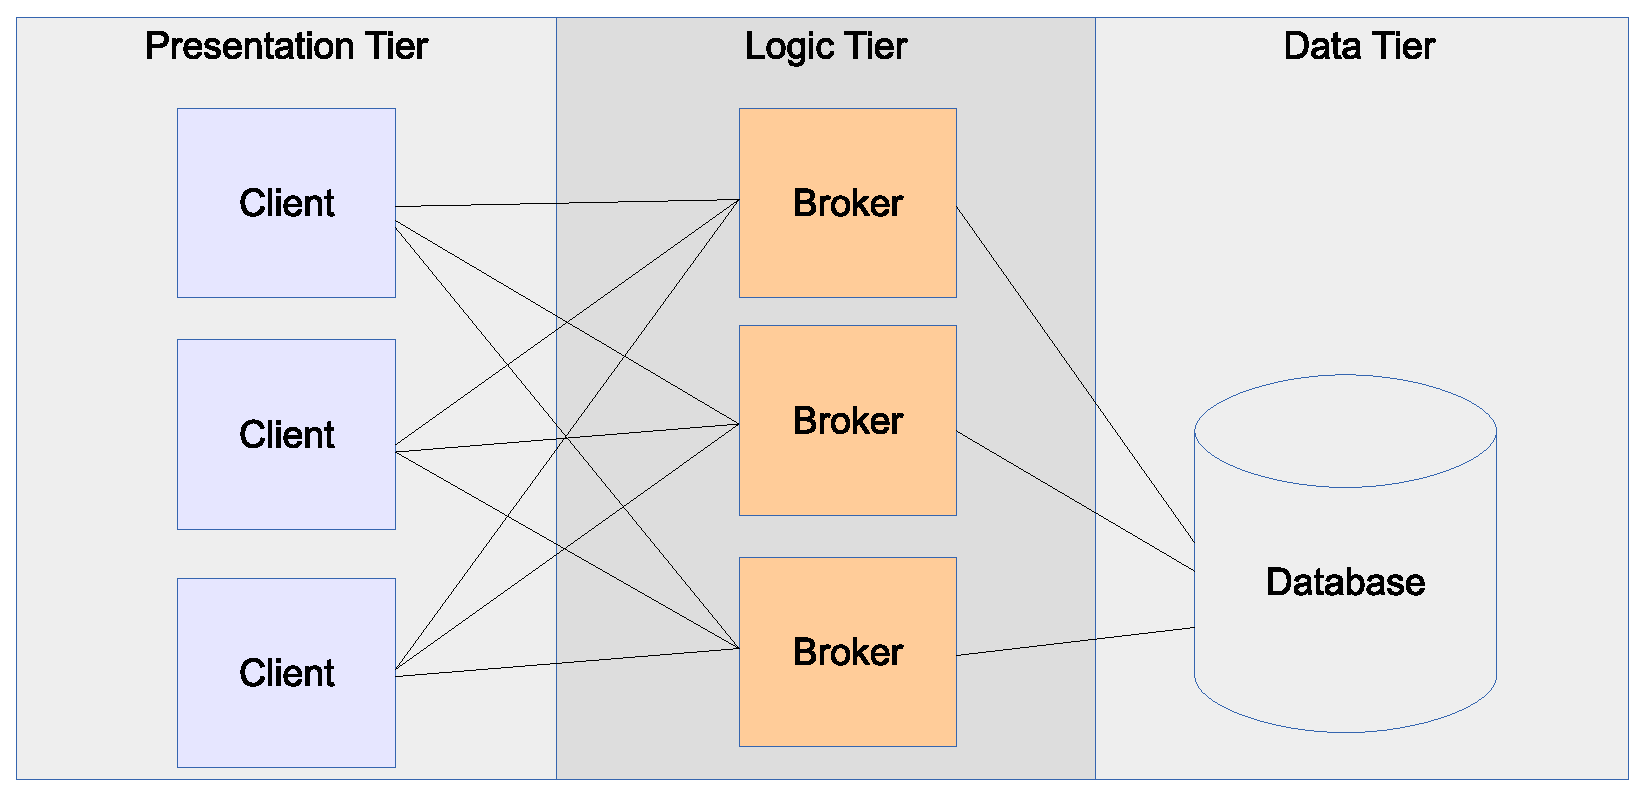
\includegraphics[scale=0.4]{../drawings/system-overview.eps}
  \end{center}
  \caption{System Overview}
  \label{fig:system-overview}
\end{figure}


%% ----------------------------------------------
\section{Messaging System}

\begin{figure}
	\begin{center}
    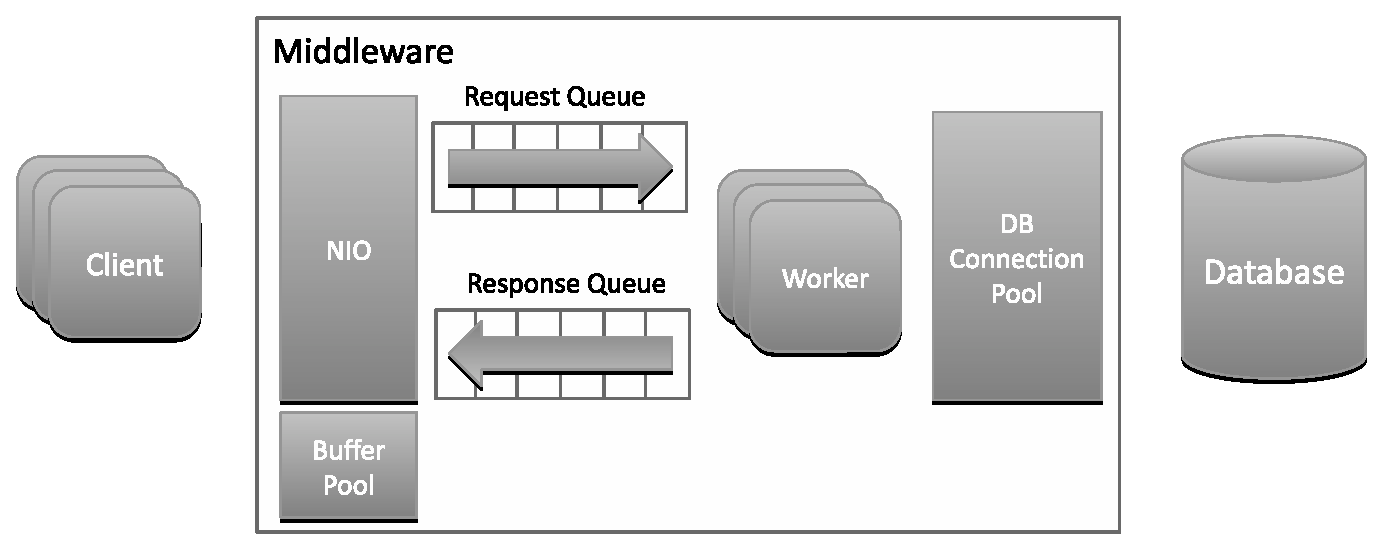
\includegraphics[scale=0.4]{../drawings/broker-threading.eps}
  \end{center}
  \caption{Middleware's main Components}
  \label{fig:middleware-threading}
\end{figure}

%% ----------------------------------------------
\section{Design Decisions}

\subsection{Schead Load}
Schead load
blocking reqeust response queues suboptimal

If queue full, immediately stop request

\subsection{NIO vs IO}

NIO VS Blocking IO

\subsection{Connection Pooling}

\subsection{Buffer Pooling}


\subsection{Message Transmission}


\section{Performance Relevant Features}

\subsection{Overview}

During a brainstorming session, a broad spectrum of performance relevant features were extracted, see figure~\ref{fig:features_mindmap}. Then, the primary features (PF, blue) and the secondary features (SF, green) were chosen according to the group membmers domain specific knowledge and presumptions.
% Later: They were then validated during discussions with other groups and the teachin assistant.


%\begin{landscape}

\tikzset{concept/.append style={fill={none}}}
\tikzset{concept/.append style={circle}}
\tikzset{level 1 concept/.append style={font=\sf, level distance = 44mm}}
\tikzset{level 2 concept/.append style={font=\sf, level distance = 22mm}}
\tikzset{level 3 concept/.append style={font=\sf, level distance = 22mm}}
\tikzset{every node/.append style={scale=0.8}}
    
\begin{figure}
\center
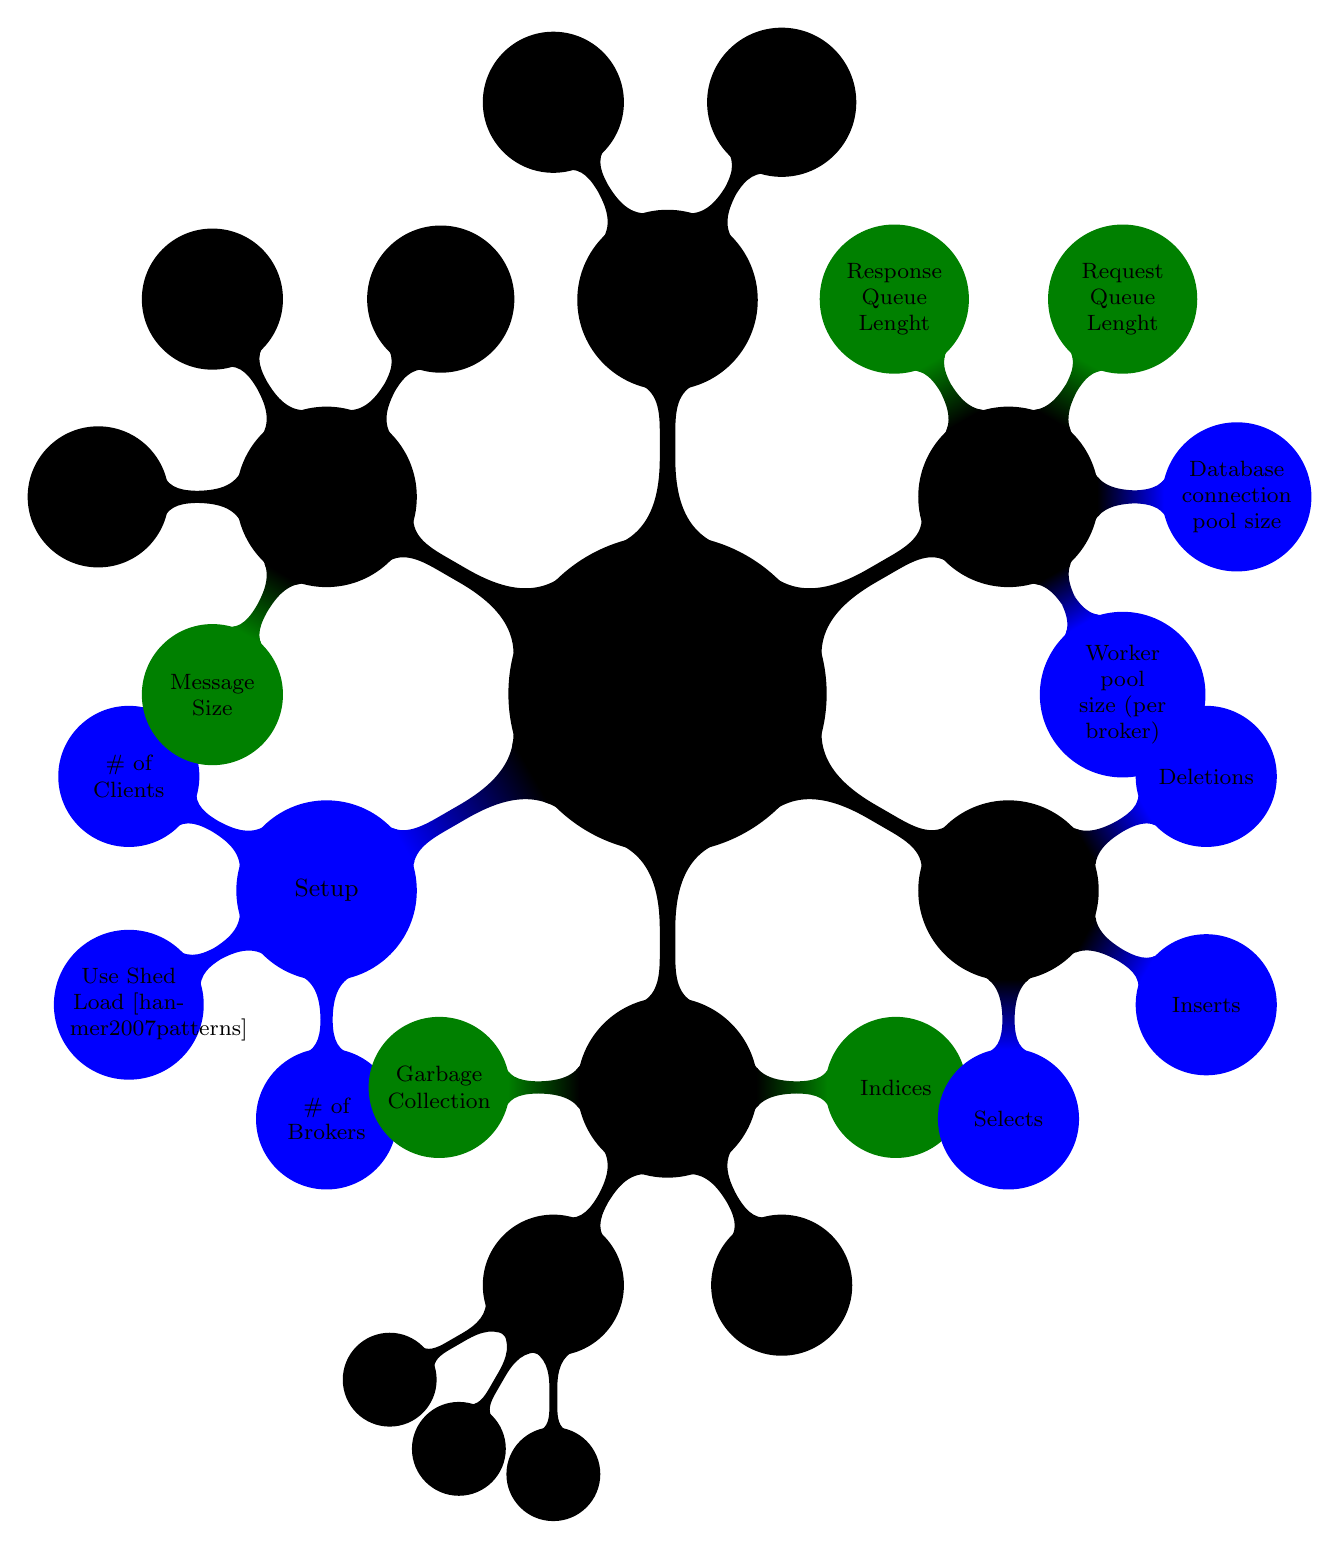
\begin{tikzpicture}[grow cyclic, align=flush center]
  \path[mindmap,concept color=black,text=black]
    node[concept] {Performance Relevant Features}
    %[clockwise from=0]
    child[concept color=blue] {
      node[concept] {Setup}
      child { 
      	node[concept] {\# of Clients} 
      }
      child {
      	node[concept] {Use Shed Load [hanmer2007patterns]} 
      }
      child {
      	node[concept] {\# of Brokers} 
      }
    }
    child[concept] {
      node[concept] {System}
      child[concept color=green!50!black] { 
        node[concept] {Garbage Collection}
      }
      child { 
        node[concept] {Hardware}
        child { node[concept] {CPU} }
        child { node[concept] {RAM} }
        child { node[concept] {Network} }
      }
      child { 
        node[concept] {Database Settings}
      }
      child[concept color=green!50!black] { node[concept] {Indices}}
    }
    child[concept] {
      node[concept] {Load types}
      child[concept color=blue] { 
      	node[concept] {Selects} 
      }
      child[concept color=blue] {
      	node[concept] {Inserts} 
      }
      child[concept color=blue] {
      	node[concept] {Deletions} 
      }
    }
    child[concept] { 
      node[concept] {Queue / Pool Sizes}
      child[concept color=blue] { 
      	node[concept] {Worker pool size (per broker)} 
      }
      child[concept color=blue] {
      	node[concept] {Database connection pool size} 
      }
      child[concept color=green!50!black] {
      	node[concept] {Request Queue Lenght} 
      }
      child[concept color=green!50!black] {
      	node[concept] {Response Queue Lenght} 
      }
    }
    child[concept] { 
      node[concept] {Logging} 
      child { 
      	node[concept] {Perfor-mance Logging} 
      }
      child {
      	node[concept] {Debug Logging} 
      }
    }
    child {
      node[concept] {Data in Database}
      child { 
      	node[concept] {\# Registered Clients} 
      }
      child {
      	node[concept] {\# Queues}
      }
      child {
      	node[concept] {\# Messages} 
      }
      child[concept color=green!50!black] {
      	node[concept] {Message Size} 
      }
    };
\end{tikzpicture}
\caption{Performance relevant features mind map} \label{fig:features_mindmap}
\end{figure}
%\end{landscape}

%% %%%%%%%%%%%%%%%%%%%%%%%%%%%%%%%%%%%%%%%%%%%%%%%%%%%%%%%%%%%%%%%%%%%%%%%%%
\section{How We Measured Our System}



\subsection{Hypothesis}

\section{References}

% TODO

http://dl.acm.org/citation.cfm?id=SERIES12798.1557393

@book{hanmer2007patterns,
  title={Patterns for fault tolerant software},
  author={Hanmer, Robert},
  year={2007},
  isbn = {0470319798, 9780470319796},
  publisher={Wiley Publishing}
}

%\bibliography{mybib}

%% %%%%%%%%%%%%%%%%%%%%%%%%%%%%%%%%%%%%%%%%%%%%%%%%%%%%%%%%%%%%%%%%%%%%%%%%%
\section{Notes - to delete}

\subsection{What should be included in this report }

\subsubsection{System Code}
\begin{itemize}
\item Code
\item Scripts for experiment
\end{itemize}

\subsubsection{Experimental data}
\begin{itemize}
\item Basic tests ans simple traces
\item Long running traces, Raw data and graphs for all experiments
\end{itemize}

\subsubsection{Written report}
\begin{itemize}
\item Architectural  diagrams
\item Interface description
\item explanation of the system design
\item Description of all experiments
\item statistical treatment of data
\item commentary analysis
\end{itemize}


\end{document}
